\documentclass[preprint,12pt,authoryear]{elsarticle}

\usepackage{amsmath,amssymb,amsthm}
\usepackage{booktabs,array}
\usepackage{graphicx}
\usepackage{url}
\usepackage{enumitem}
\usepackage{microtype}
\usepackage{placeins}
\usepackage[labelfont=bf]{caption}
\usepackage{subcaption}
\usepackage{xr-hyper}
\usepackage[colorlinks=true,linkcolor=blue,citecolor=blue,urlcolor=blue]{hyperref}

\journal{Epidemics}

\newtheorem{sproposition}{Supplementary Proposition}
\renewcommand{\thesproposition}{S\arabic{sproposition}}

\newcommand{\E}{\mathbb{E}}
\newcommand{\Var}{\mathrm{Var}}
\newcommand{\Cov}{\mathrm{Cov}}
\newcommand{\NB}{\mathrm{NB}}
\newcommand{\Bin}{\mathrm{Bin}}
\newcommand{\CV}{\mathrm{CV}}
\newcommand{\Rbar}{\bar{R}}
\newcommand{\mx}{m_\times}

\externaldocument{build/main}

\renewcommand{\thesection}{S\arabic{section}}
\renewcommand{\thesubsection}{S\arabic{section}.\arabic{subsection}}
\renewcommand{\theequation}{S\arabic{equation}}
\renewcommand{\thetable}{S\arabic{table}}
\renewcommand{\thefigure}{S\arabic{figure}}

\begin{document}

\begin{frontmatter}

\title{Supplementary Material: Limits to improving reproduction number estimates by increasing case counts: Environmental variability, reporting heterogeneity, and surveillance design}

\author{Chi Wang}
\affiliation{organization={School of Safety Science and Engineering, Xi'an University of Science and Technology},
            city={Xi'an},
            postcode={710054},
            country={China}}

\end{frontmatter}

\section{Mathematical proofs and analytical derivations}
\label{app:proofs}

This section provides complete mathematical proofs for all propositions, corollaries, and remarks in the main text, alongside detailed derivations of the renewal process variance decompositions and higher-order delta expansions. Equation and theorem numbering from the main text is preserved; equations introduced solely in this supplement carry the prefix S.

Recall that the negative-binomial distribution $\NB(r, p)$ parameterized by number of failures $r$ and success probability $p$ has mean $r(1-p)/p$ and variance $r(1-p)/p^2$. Setting $r = k$ and $p = k/(k + R)$ yields Eq.~\eqref{eq:offspring}. Convolutions and binomial thinning follow directly from infinite divisibility and thinning properties of the negative-binomial family \citep{casella2002statistical}.

\subsection{Proof of Proposition 1 (Estimation of Target 1)}
\label{sec:proof-prop1}

Let $c$ denote an observed realization of $C_t$, and let $\theta = \rho R_t$. From Eq.~\eqref{eq:observed}, the conditional log-likelihood of $R_t$ given $n$ is
\begin{equation}
  \ell(R_t) = \text{const} + nk\log\left(\frac{k}{k+\theta}\right) + c\log\left(\frac{\theta}{k+\theta}\right).
\end{equation}
Differentiating with respect to $R_t$, the score function is
\begin{equation}
  \dot{\ell}(R_t) = \frac{c}{R_t} - \frac{(c+nk)\rho}{k+\rho R_t}
  = \mathcal{I}(R_t)\,(\widehat{R}_t - R_t), \qquad
  \mathcal{I}(R_t) = \frac{k\rho n}{R_t(k+\rho R_t)} = \frac{n}{R_t/\rho + R_t^2/k}.
  \label{eq:score}
\end{equation}

\begin{enumerate}[label=(\roman*)]
  \item When $c > 0$, Eq.~\eqref{eq:score} implies $\dot{\ell}(R_t) > 0$ for $R_t < \widehat{R}_t$ and $\dot{\ell}(R_t) < 0$ for $R_t > \widehat{R}_t$. Hence, the log-likelihood is strictly concave and achieves its unique global maximum at $\widehat{R}_t = c/(\rho n)$. When $c = 0$, $\dot{\ell}(R_t) = -nk\rho/(k+\rho R_t) < 0$ for all $R_t > 0$, so the maximum is attained at the boundary $R_t = 0 = \widehat{R}_t$.
  \item Conditional expectation is $\E(\widehat{R}_t \mid R_t) = \rho n R_t / (\rho n) = R_t$, proving unbiasedness. Conditional variance is
  \begin{equation}
    \Var(\widehat{R}_t \mid R_t) = \frac{\rho n R_t + \rho^2 n R_t^2 / k}{(\rho n)^2} = \frac{R_t}{\rho n} + \frac{R_t^2}{kn} = \frac{R_t(k+\rho R_t)}{k\rho n}.
  \end{equation}
  \item The Fisher information is the variance of the score function:
  \begin{equation}
    \mathcal{I}(R_t) = \Var(\dot{\ell}(R_t)) = \frac{(k\rho n)^2}{[R_t(k+\rho R_t)]^2}\Var(\widehat{R}_t) = \frac{k\rho n}{R_t(k+\rho R_t)} = \frac{n}{R_t/\rho + R_t^2/k}.
  \end{equation}
  Thus, $\Var(\widehat{R}_t \mid R_t) = 1/\mathcal{I}(R_t)$. Because the score function is strictly proportional to $\widehat{R}_t - R_t$, equality in the Cram\'er--Rao inequality is attained for all finite $n$ \citep{casella2002statistical}.
  \item Writing the probability mass function of Eq.~\eqref{eq:observed} in natural exponential family form, the natural parameter is $\upsilon = \log[\rho R_t / (k+\rho R_t)]$. As $R_t \in (0, \infty)$, $\upsilon$ spans $(-\infty, 0)$, which contains an open interval. Therefore, $C_t$ is a complete sufficient statistic. Because $\widehat{R}_t$ is an unbiased function of $C_t$, by the Lehmann--Scheff\'e theorem it is the unique uniformly minimum-variance unbiased estimator (UMVUE) \citep{lehmann2005testing}. \qed
\end{enumerate}

\subsection{Proof of Proposition 2 (Estimation of Target 2)}
\label{sec:proof-prop2}

Under H4, $\E(R_t \mid n) = \Rbar$ and $\Var(R_t \mid n) = v_R$. By Proposition~\ref{prop:current}, $\E(\widehat{R}_t \mid n, R_t) = R_t$, so $\E(\widehat{R}_t \mid n) = \Rbar$. By the law of total variance:
\begin{align}
  \Var(\widehat{R}_t \mid n) &= \E\big[\Var(\widehat{R}_t \mid n, R_t)\mid n\big] + \Var\big[\E(\widehat{R}_t \mid n, R_t)\mid n\big] \nonumber \\
  &= \E\left[\frac{R_t}{\rho n} + \frac{R_t^2}{kn}\ \Big|\ n\right] + \Var(R_t \mid n) \nonumber \\
  &= \frac{\Rbar}{\rho n} + \frac{\Rbar^2 + v_R}{kn} + v_R.
\end{align}
Substituting $m = \rho n$ and collecting terms in $1/m$ yields Eq.~\eqref{eq:var-average}.
\begin{enumerate}[label=(\roman*)]
  \item As $m \to \infty$, $A/m \to 0$, hence $V(m) \to v_R$.
  \item The sampling fraction of total variance is $(A/m)/(v_R + A/m) = 1/(1 + m v_R / A) = 1/(1 + m/m_\times)$.
  \item Proportional variance reduction upon doubling sample size is $[V(m) - V(2m)]/V(m) = [A/(2m)]/(v_R + A/m) = 1/[2(1 + m/m_\times)]$.
  \item $V'(m) = -A/m^2 < 0$ and $V''(m) = 2A/m^3 > 0$, proving strict monotonicity and convexity. The scale elasticity is $\epsilon_m = m V'(m)/V(m) = -(A/m)/(v_R + A/m) = -m_\times / (m + m_\times)$, which evaluates to $-1/2$ at $m = m_\times$.
  \item Let $\tilde{\theta}$ be any estimator based on current-period data satisfying $\E(\tilde{\theta} \mid R_t) = R_t$. By the Cram\'er--Rao inequality, $\Var(\tilde{\theta} \mid R_t) \ge 1/\mathcal{I}(R_t)$. Substituting into the orthogonal decomposition $\E(\tilde{\theta} - \Rbar)^2 = \E[\Var(\tilde{\theta} \mid R_t)] + v_R \ge v_R + \E[1/\mathcal{I}(R_t)] = V(m)$, with equality achieved by $\widehat{R}_t$. For one-step forecasting, $y = C_{t+1}/m$. By H4, $R_{t+1}$ is independent of $\mathcal{F}_t$, so $\E[(\hat{y} - y)^2 \mid \mathcal{F}_t] = (\hat{y} - \E y)^2 + \Var(y) \ge \Var(y) = V(m)$, with equality attained at $\hat{y} = \Rbar$. \qed
\end{enumerate}

\subsection{Derivation of Remark 1 (Reporting completeness versus coverage)}
\label{sec:proof-rem1}

Writing $V(n, \rho) = v_R + \Rbar/(\rho n) + (\Rbar^2 + v_R)/(kn)$:
\begin{equation}
  \lim_{\rho \to 1} V(n, \rho) = v_R + \frac{\Rbar}{n} + \frac{\Rbar^2 + v_R}{kn} > v_R, \qquad
  \lim_{n \to \infty} V(n, \rho) = v_R.
\end{equation}
Evaluating log-marginal effects:
\begin{equation}
  -\frac{\partial V}{\partial \log n} = \frac{\Rbar}{\rho n} + \frac{\Rbar^2 + v_R}{kn} = \frac{A}{m}, \qquad
  -\frac{\partial V}{\partial \log \rho} = \frac{\Rbar}{\rho n} = \frac{\Rbar}{m}.
\end{equation}
Their ratio is $A/\Rbar = 1 + \rho(\Rbar^2 + v_R)/(k\Rbar)$.

\subsection{Proof of Proposition 5 (Multi-period allocation and cost optimization)}
\label{sec:proof-prop5}

\begin{enumerate}[label=(\roman*)]
  \item Under H1--H4 with equal ancestor volume $n$ per period, conditional on $(R_1, \dots, R_T)$, counts across periods are independent. Letting $\bar{R}_T = T^{-1}\sum_{t=1}^T R_t$, by the law of total variance:
  \begin{equation}
    \frac{1}{T^2}\Var\Bigl(\sum_{t=1}^T \widehat{R}_t\Bigr) = \Var(\bar{R}_T) + \frac{1}{T^2}\sum_{t=1}^T \E\left[\frac{R_t}{\rho n} + \frac{R_t^2}{kn}\right] = \Var(\bar{R}_T) + \frac{A}{Tm}.
  \end{equation}
  The second term equals $A/B$, depending solely on total sample size $B = Tm$. When $R_t$ is i.i.d., $\Var(\bar{R}_T) = v_R/T$, yielding Eq.~\eqref{eq:alloc-indep}.
  Under a stationary AR(1) process with $\Cov(R_s, R_t) = v_R \phi^{|s-t|}$, we have
  \begin{equation}
    T^2\Var(\bar{R}_T) = v_R T + 2v_R \sum_{h=1}^{T-1}(T-h)\phi^h = v_R\left[\frac{T(1+\phi)}{1-\phi} - \frac{2\phi(1-\phi^T)}{(1-\phi)^2}\right],
  \end{equation}
  which can be verified by induction on $T$. Strict monotonicity in $T$ follows from the concavity of partial sums of geometric series.
  \item Substituting $T = \mathcal{B}/(c_0 + c_1m)$ into Eq.~\eqref{eq:alloc-indep}:
  \begin{equation}
    f(m) = \frac{(c_0 + c_1m)(v_R + A/m)}{\mathcal{B}} = \frac{c_0v_R + c_1A + c_1v_Rm + c_0A/m}{\mathcal{B}}.
  \end{equation}
  Differentiating yields $f'(m) = (c_1v_R - c_0A/m^2)/\mathcal{B}$ and $f''(m) = 2c_0A/(m^3\mathcal{B}) > 0$. For $c_0 > 0$, $f$ is strictly convex on $(0, \infty)$, with unique stationary point $m^{*2} = c_0A/(c_1v_R) = (c_0/c_1)m_\times$. Substituting $m^*$ yields Eq.~\eqref{eq:optimal-m}. \qed
\end{enumerate}

\subsection{Proof of Outbreak Detection Test Properties}
\label{sec:proof-test}

For $R > R'$, the likelihood ratio from Eq.~\eqref{eq:observed} is
\begin{equation}
  \frac{f(c; R)}{f(c; R')} = \frac{(k+\rho R')^{nk}\,[R(k+\rho R')]^{c}}{(k+\rho R)^{nk}\,[R'(k+\rho R)]^{c}}.
\end{equation}
Because $R/(k+\rho R)$ is strictly increasing in $R$, the base $R(k+\rho R')/[R'(k+\rho R)] > 1$. Thus, the likelihood ratio is strictly increasing in $c$, establishing that the family possesses a monotone likelihood ratio (MLR) in $C_t$.

\begin{enumerate}[label=(\alph*)]
  \item \textbf{Size:} By standard MLR theory, the power function of any test of the form $\{C_t \ge c\}$ is non-decreasing in $R_t$ \citep{lehmann2005testing}. Hence, the maximum rejection probability on $H_0\colon R_t \le 1$ is attained at $R_t = 1$, where it equals $\alpha^* = P_{R_t=1}(C_t \ge c_\alpha) \le \alpha$.
  \item \textbf{Uniform optimality:} By the Karlin--Rubin theorem \citep{karlin1956theory}, the test rejecting when $C_t \ge c_\alpha$ is uniformly most powerful (UMP) at level $\alpha^*$.
  \item \textbf{Power:} Under $R_t = 1 + \delta$, $C_t \sim \NB(nk, k/[k+\rho(1+\delta)])$, yielding Eq.~\eqref{eq:power}. \qed
\end{enumerate}

\subsection{Proof of Proposition 3 and Corollary 1 (Reporting Heterogeneity)}
\label{sec:proof-prop3}

\begin{enumerate}[label=(\roman*)]
  \item Given $(n, R_t, p_t)$, $\E(C_t \mid \cdot) = p_t n R_t$ and $\Var(C_t \mid \cdot) = p_t n R_t + p_t^2 n R_t^2 / k$. Applying the law of total variance over $p_t$, and using $\E p_t = \rho$ and $\E p_t^2 = \rho^2 + \sigma^2$:
  \begin{equation}
    \Var(C_t \mid n, R_t) = \rho n R_t + \frac{(\rho^2+\sigma^2)nR_t^2}{k} + \sigma^2 n^2 R_t^2.
  \end{equation}
  \item Unbiasedness follows from $\E(C_t \mid n, R_t) = \rho n R_t$, so $\E \widehat{R}_t = \Rbar$. Applying total variance over $R_t$ and dividing by $(\rho n)^2$:
  \begin{equation}
    V_H(m) = v_R + \frac{\sigma^2}{\rho^2}(\Rbar^2 + v_R) + \frac{\Rbar}{m} + \frac{(\rho^2+\sigma^2)(\Rbar^2+v_R)}{\rho km},
  \end{equation}
  which yields Eq.~\eqref{eq:r3-vH} with $v_H = \tau^2(\Rbar^2 + v_R)$.
  \item Let $\theta_t = p_t R_t = \rho R_t u_t$. The Markov chain $R_t \to \theta_t \to C_t$ and the data processing inequality for Fisher information \citep{zamir1998proof} yield $\mathcal{I}_{C_t}(R_t) \le \mathcal{I}_{\theta_t}(R_t) = \mathcal{J}_u / R_t^2$, where $\mathcal{J}_u$ is the scale information of $u_t$. By Cauchy--Schwarz, $\mathcal{J}_u \ge 1/\tau^2$, with equality attained if and only if $u_t$ follows a Gamma distribution with shape and rate $1/\tau^2$.
  \item Unidentifiability: Note that $v_R + v_H = U - \Rbar^2$ and $A_H = \Rbar + \rho U / k$, where $U = (1+\tau^2)(\Rbar^2+v_R)$. The marginal distribution of $(C_1, \dots, C_T)$ up to second moments depends on $(v_R, \tau^2)$ exclusively through the scalar combination $U$.
  \item Denominator lag signature: Let $D_t = \sum_s w_s C_{t-s}$. Under AR(1) reporting shock $u_t = 1 + \epsilon_t$ with persistence $\psi$, first-order delta expansion yields Eq.~\eqref{eq:r3-Fw}. Evaluating $F(w, \psi)/F(w', \psi)$ across $\psi \in [0, 1)$ yields the analytical bounds $q_1 \in [0.883, 1.338]$ and $q_2 \in [0.892, 1.374]$. \qed
\end{enumerate}

For Corollary~\ref{cor:switch}, differentiating $V_H$ with respect to $\log\rho$ and $\log n$:
\begin{equation}
  -\rho\frac{\partial V_H}{\partial \rho} - \left(-n\frac{\partial V_H}{\partial n}\right) = \frac{\Rbar^2+v_R}{kn}\left[-\rho\frac{\mathrm{d}\tau^2}{\mathrm{d}\rho}(kn+1) - (1+\tau^2)\right].
\end{equation}
Under institutional reporting ($\mathrm{d}\tau^2/\mathrm{d}\rho = 0$), the difference is strictly negative. Under binomial reporting ($\tau^2 = (1-\rho)/[\rho(\nu+1)]$), setting the bracket positive yields $kn > \rho\nu \iff m > \rho^2\nu/k$. \qed

\subsection{Proof of Proposition 6 (Precision of Environmental Variance Estimation)}
\label{sec:proof-prop6}

\begin{sproposition}[Finite-period precision and Fisher information for environmental variance]
\label{sprop:vR-finite}
Under H1--H4 and H6, with equal sample volume $m$ per period:
\begin{enumerate}[label=(\alph*)]
  \item When $R_t$ is i.i.d., the modified moment estimator $\hat{v}_R$ in Eq.~\eqref{eq:r3-vhat} has bias $-\rho\sigma_Y^2/[kmT(1+\rho/(km))]$ and variance
  \begin{equation}
    \Var(\hat{v}_R) = \frac{1}{(1+\rho/(km))^2}\left[\frac{\mu_{4Y}}{T} - \frac{(T-3)\sigma_Y^4}{T(T-1)} - \frac{2\varpi'\mu_{3Y}}{T} + \frac{\varpi'^2\sigma_Y^2}{T}\right]\left(1 + O\left(\frac{1}{mT}\right)\right),
    \label{eq:r3-omega}
  \end{equation}
  where $\varpi' = (1 + 2\rho\bar{R}/k)/m$. As $m \to \infty$, $T\Var(\hat{v}_R) \to \Omega_\infty = \E(R_t-\bar{R})^4 - v_R^2$. When $R_t \sim \text{Gamma}(\xi, \vartheta)$, $\Omega_\infty = v_R^2(2 + 6v_R/\bar{R}^2)$.
  \item Let the joint distribution of $(R_1, \dots, R_T)$ belong to a family parameterized by $v_R$. For any scale $m$ and any correlation structure, $\mathcal{I}_{C_{1:T}}(v_R) \le \mathcal{I}_{R_{1:T}}(v_R)$. When periods are independent with $R_t \sim \text{Gamma}$ of fixed mean $\bar{R}$:
  \begin{equation}
    \mathcal{I}_{R_{1:T}}(v_R) = \frac{T\xi\,[\xi(\ln\Gamma)''(\xi) - 1]}{v_R^2}, \qquad \xi = \frac{\bar{R}^2}{v_R},
    \label{eq:r3-IR}
  \end{equation}
  where $(\ln\Gamma)''$ is the trigamma function. For stationary Gaussian AR(1) environments, $\mathcal{I}_{R_{1:T}}(v_R) = T/(2v_R^2)$, independent of $\phi$.
\end{enumerate}
\end{sproposition}

\begin{proof}
Item (i) in Proposition~\ref{prop:vR-info} follows from setting sample variance $S_C^2$ equal to marginal variance $m^2 V(m) = m^2 v_R + m\bar{R} + (\rho m/k)(\bar{R}^2+v_R)$ and solving for $v_R$.

For Supplementary Proposition~\ref{sprop:vR-finite}(a), standard moments of sample variance give Eq.~\eqref{eq:r3-omega}. As $m \to \infty$, $Y_t \to R_t$, recovering $\Omega_\infty = \Var((R_t-\bar{R})^2) = \E(R_t-\bar{R})^4 - v_R^2$. For $\text{Gamma}(\xi, \vartheta)$, the fourth central moment is $3\xi(\xi+2)\vartheta^4$, which upon substituting $\xi = \bar{R}^2/v_R$ and $\vartheta = v_R/\bar{R}$ yields $\Omega_\infty = v_R^2(2 + 6v_R/\bar{R}^2)$.

For Supplementary Proposition~\ref{sprop:vR-finite}(b), the Markov chain $v_R \to R_{1:T} \to C_{1:T}$ and the data processing inequality yield $\mathcal{I}_{C_{1:T}}(v_R) \le \mathcal{I}_{R_{1:T}}(v_R)$. Evaluating the Fisher information matrix for the two-parameter Gamma family under the chain rule $\mathrm{d}\xi/\mathrm{d}v_R = -\bar{R}^2/v_R^2$ and $\mathrm{d}\vartheta/\mathrm{d}v_R = 1/\bar{R}$ yields Eq.~\eqref{eq:r3-IR}. Under stationary Gaussian AR(1), $R_{1:T} - \bar{R} \sim \mathcal{N}(0, v_R \Sigma_\phi)$, giving Fisher information $\frac{1}{2}\mathrm{tr}\{[(v_R \Sigma_\phi)^{-1}\Sigma_\phi]^2\} = T/(2v_R^2)$.

Finally, for Gaussian AR(1), $\Cov[(R_s-\bar{R})^2, (R_t-\bar{R})^2] = 2v_R^2 \phi^{2|s-t|}$. Summing over pairs yields $2v_R^2 \kappa_T(\phi^2)/T$, confirming Eq.~\eqref{eq:r3-teff}.
\end{proof}

\subsection{Proof of Corollary 2 (Season-Level Variance Bound)}
\label{sec:proof-cor2}

Forming the Markov chain $v_S \to (\eta_1, \dots, \eta_S) \to (R_t) \to (C_t)$, the data processing inequality establishes that the total Fisher information for $v_S$ cannot exceed the information in the latent seasonal shocks: $\mathcal{I}(v_S) \le S/(2v_S^2)$. By Cram\'er--Rao, any unbiased estimator satisfies $\Var(\hat{v}_S) \ge 2v_S^2/S$, proving the $\sqrt{2/S}$ relative error bound. When seasonal means are unknown, sample variance degrees of freedom reduce to $S-1$. \qed

\subsection{Proof of Proposition 7 (Budget Threshold under AR(1) Environments)}
\label{sec:proof-prop7}

Substituting the budget constraint into $f_\phi(T) = v_R e(T) + A c_1 / (\mathcal{B} - c_0 T)$, the first-order condition requires $v_R g_T = c_0 A / (c_1 m^2)$. Monotonicity of $g_T(\phi)$ from $g_1 < 1$ to $(1+\phi)/(1-\phi) > 1$ guarantees a unique root $T^\dagger$ where $g_{T^\dagger} = 1$, corresponding to budget $\mathcal{B}^\dagger = T^\dagger(c_0 + c_1 m_0^*)$. When $\mathcal{B} < \mathcal{B}^\dagger$, $T^* < T^\dagger$ and $g_{T^*} < 1$, requiring $m^* > m_0^*$. When $\mathcal{B} > \mathcal{B}^\dagger$, $m^* < m_0^*$. \qed

\subsection{Shrinkage and Empirical Bayes Estimation}
\label{sec:proof-shrink}

Consider the linear shrinkage estimator $\hat{\theta}_\lambda = (1-\lambda)C_t/m + \lambda\mu_0$, where $\mu_0$ is a prior benchmark and $\delta = \mu_0 - \Rbar$. The mean squared error is
\begin{equation}
  \mathrm{MSE}(\lambda) = (1-\lambda)^2 V + \lambda^2 \delta^2, \qquad V = v_R + \frac{A}{m}.
\end{equation}
Minimizing over $\lambda$ yields $\lambda^* = V/(V+\delta^2)$ and $\mathrm{MSE}(\lambda^*) = V\delta^2 / (V+\delta^2)$. Thus, $\mathrm{MSE}(\lambda^*) < v_R$ if and only if $\delta^2 < v_R(1 + m/m_\times)$. The estimator achieves variance reduction by introducing conditional bias $\lambda(\mu_0 - R_t)$. \qed

\subsection{Renewal Process Variance and Delta Expansion of Denominator Noise}
\label{sec:proof-renewal}

Conditional on history $\mathcal{F}_t$, let $\bar{\Lambda} = \E(\Lambda_{t+1} \mid \mathcal{F}_t)$ and $m = \rho \bar{\Lambda}$. By the law of total variance conditioned on $(\Lambda_{t+1}, R_{t+1})$:
\begin{align}
  \Var(C_{t+1} \mid \mathcal{F}_t) &= \E\left[\rho \Lambda_{t+1} R_{t+1} + \frac{\rho^2 \Lambda_{t+1} R_{t+1}^2}{k}\ \Big|\ \mathcal{F}_t\right] + \Var(\rho \Lambda_{t+1} R_{t+1} \mid \mathcal{F}_t) \nonumber \\
  &= m A + \rho^2 \bar{\Lambda}^2 \left[v_R + \CV^2(\Lambda_{t+1} \mid \mathcal{F}_t)\,(\Rbar^2 + v_R)\right].
\end{align}
Dividing by $m^2 = (\rho \bar{\Lambda})^2$ yields Eq.~\eqref{eq:info-decomp}.

For the denominator noise expansion, condition on true infection history $\mathcal{H}_t$, and define $D_t = m(1+\delta)$ where $m = \rho \Lambda_{t+1}$ and $c_w = (1-\rho)\sum_s w_s^2$. Then $\E(\delta) = 0$ and $\E(\delta^2) = c_w/m$. Expanding $G_t = (C_{t+1}/m)(1+\delta)^{-1}$ to second order in $\delta$:
\begin{equation}
  \E(G_t \mid \mathcal{H}_t) = \Rbar\left(1 + \frac{c_w}{m}\right) + O(m^{-2}), \qquad
  \Var(G_t \mid \mathcal{H}_t) = v_R + \frac{A + (\Rbar^2 + 3v_R)c_w}{m} + O(m^{-2}).
\end{equation}
Normalizing by the squared conditional expectation $[\E(G_t \mid \mathcal{H}_t)]^2 = \Rbar^2[1 + 2c_w/m + O(m^{-2})]$ eliminates $2v_R c_w/m$, yielding the slope expression in Eq.~\eqref{eq:b-delta}. \qed


\section{Robustness analyses and supplementary tables}
\label{sec:s-robust}

This section documents the robustness checks, sensitivity specifications, and supplementary tables referenced in the main text.

\subsection{Equivalence testing of reporting adjustment}
\label{sec:s-tost}

Table~\ref{tab:s-tost} presents the two one-sided tests for equivalence (TOST) evaluating the impact of reporting completeness adjustment $\Delta a = a - a^*$ across seven pathogen-window combinations. All three influenza combinations demonstrate statistical equivalence under both BCa bootstrap intervals and normal approximation tests at the 5\% margin ($\pm 0.0050$). Calendar windows for COVID-19 and RSV achieve equivalence under the BCa interval criterion. The two growth-phase windows exceed equivalence margins primarily because their baseline intercepts are small ($a \approx 0.02$--$0.03$), making the 5\% equivalence band extremely narrow ($\pm 0.001$). For the 2025--2026 influenza season, $\Delta a = +0.0039$ (90\% BCa CI 0.0020--0.0060), which remains within the seasonal equivalence margin of 0.0088.

\subsection{Evaluation of reporting detection power on simulated grids}
\label{sec:s-tau}

Table~\ref{tab:s-tau} evaluates the sensitivity of the $\Delta a$ detection metric across a 35-cell simulation grid of reporting volatility. When reporting fluctuations are uncorrelated with hospital reporting completeness ($\kappa = 0$), the false rejection rate is 0 across all cells. As elasticity $\kappa$ increases, power to detect reporting effects rises; however, because empirical reporting completeness is concentrated near unity (median 0.943), observable institutional completeness explains $<1\%$ of intercept elevation, while within-facility underreporting or clinical threshold shifts ($\tau > 0$) remain unconstrained by $\Delta a$.

\subsection{Epidemic season random-effects pooling}
\label{sec:s-seasons}

Table~\ref{tab:s-seasons} reports season-specific intercept estimates and random-effects pooling using the DerSimonian--Laird method. Individual season intercepts range from 0.028 to 0.135 ($Q = 47.4, p = 5\times 10^{-11}$). The pooled intercept across the three primary seasons is $a_{\mathrm{RE}} = 0.077$ (95\% CI $-0.056$ to $0.211$; $\hat{v}_S = 0.0028$), illustrating the theoretical precision lower bound $\sqrt{2/(S-1)} = 1.00$ for $S = 3$.

\subsection{Generation interval aggregation sensitivity}
\label{sec:s-twogen}

Table~\ref{tab:s-twogen} evaluates sensitivity to discrete generation block length (7 days versus 4 days). Decreasing block length scales baseline intercept magnitude down to approximately 60\% under independent environments, but intercept ratios $q_1, q_2$ vary by less than 0.05. Intercept ratios are driven primarily by admission delay convolution rather than generation block aggregation.

\subsection{Independent non-NHSN surveillance streams}
\label{sec:s-indep}

Table~\ref{tab:s-indep} presents scaling estimates from outpatient ILINet ($N = 1{,}479$) and hospital FluSurv-NET ($N = 364$). ILINet reproduces the directional intercept pattern ($q_1 = 0.687, q_2 = 1.467$, with 99.7\% of bootstrap resamples satisfying $q_1 < 1 < q_2$). FluSurv-NET covers only 14 sentinel sites, producing wide confidence intervals that span unity.

\subsection{Null range specifications and evidence grading}
\label{sec:s-grading}

Table~\ref{tab:s-grading} details pre-registered null simulation ranges and sensitivity classifications across the seven pathogen-window combinations. Under pre-registered full-grid criteria, 4 combinations achieve partial replication and 3 show directional consistency (0/4/3). Under sensitivity specifications excluding admission delays, full replication is achieved in 2 combinations.

\subsection{Supplementary figures}
\label{sec:s-figs}

\begin{figure}[!tbp]
  \centering
  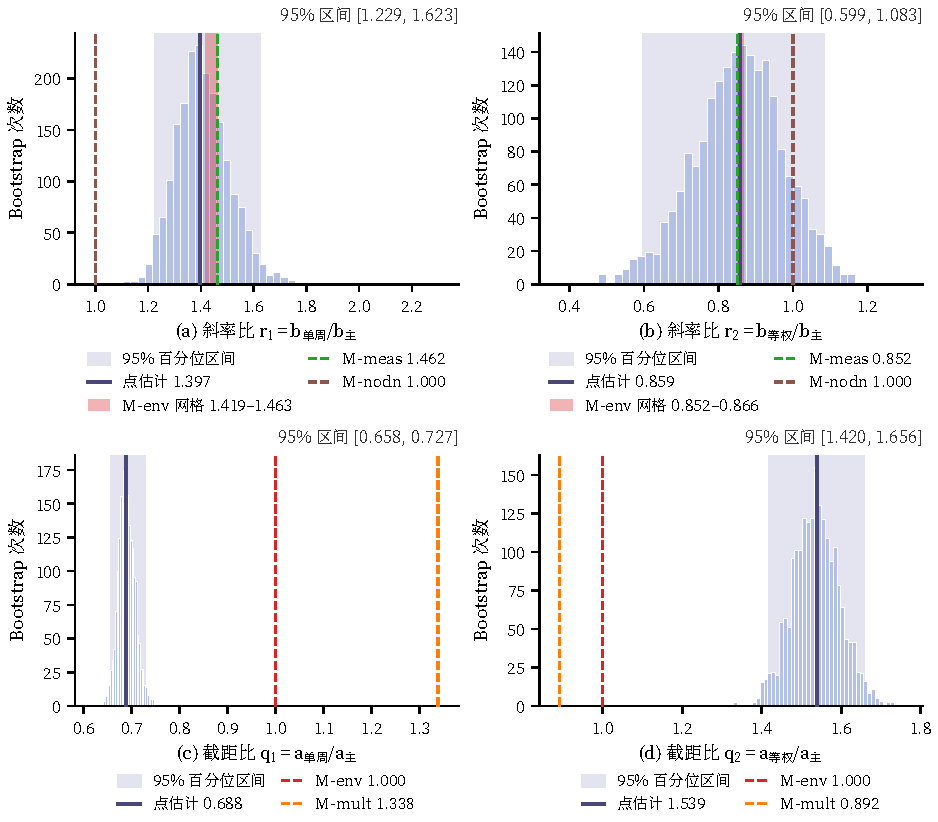
\includegraphics[width=\textwidth]{figures/fig_s1_bootstrap.pdf}
  \caption{State-clustered bootstrap distributions of lag-weight ratios ($N = 1{,}267$ state-weeks, $B = 2{,}000$ resamples). (A) Slope ratio $r_1 = b_{\mathrm{single}} / b_{\mathrm{primary}}$. (B) Slope ratio $r_2 = b_{\mathrm{equal}} / b_{\mathrm{primary}}$. (C) Intercept ratio $q_1 = a_{\mathrm{single}} / a_{\mathrm{primary}}$. (D) Intercept ratio $q_2 = a_{\mathrm{equal}} / a_{\mathrm{primary}}$. Vertical solid lines indicate point estimates; grey shaded areas represent 95\% percentile confidence intervals; tick markers indicate theoretical predictions from candidate mechanisms (Table~\ref{tab:ratios}). Slope ratios exclude the noise-free denominator model (M-nodn), while intercept ratios reject stationary models but overlap with dynamic growth renewal ranges.}
  \label{fig:s-boot}
\end{figure}

\begin{figure}[!tbp]
  \centering
  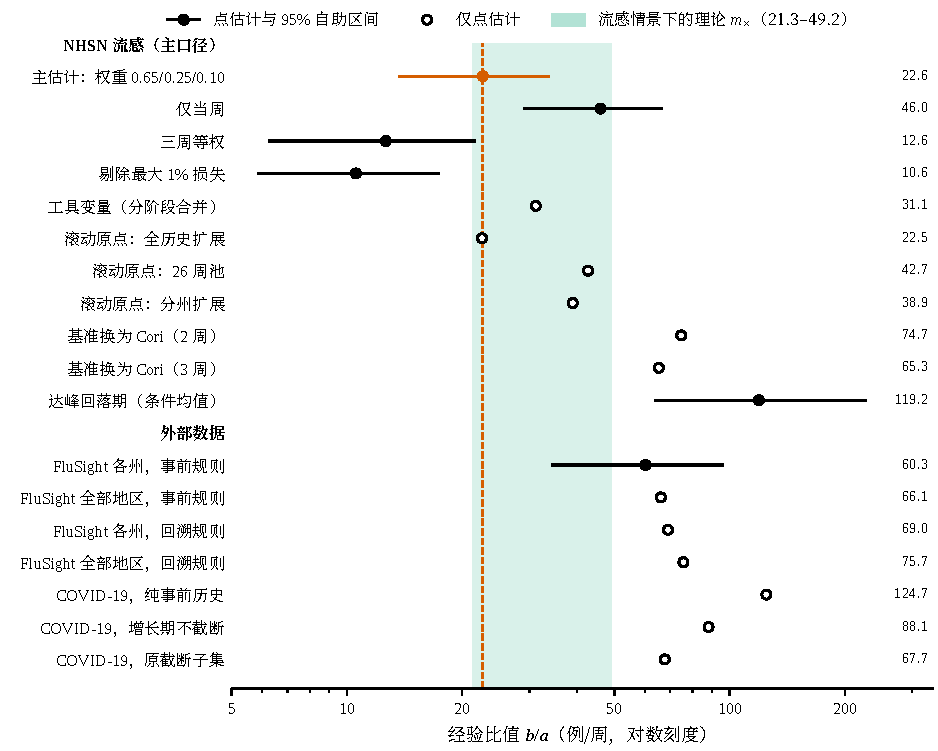
\includegraphics[width=0.96\textwidth]{figures/fig_s2_forest.pdf}
  \caption{Forest plot of empirical balance scale ratios $b/a$ across model specifications (cases/week, logarithmic scale). Horizontal bars represent 95\% confidence intervals from cluster bootstrap resamples. Shaded band indicates the theoretical scenario range $m_\times \in [21.3, 49.2]$, with vertical dashed line marking the baseline estimate of 22.6 cases/week. Upper section displays NHSN influenza sensitivity specifications; lower section displays external surveillance streams.}
  \label{fig:s-forest}
\end{figure}

\begin{figure}[!tbp]
  \centering
  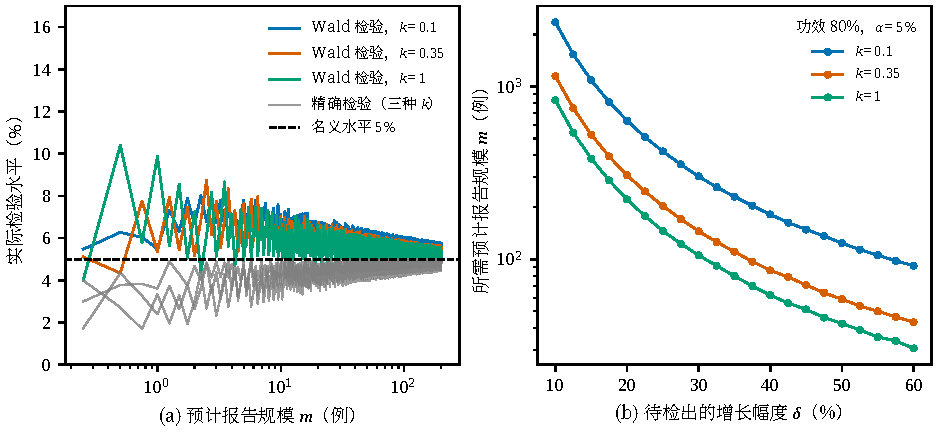
\includegraphics[width=\textwidth]{figures/fig_s3_growth.pdf}
  \caption{Exact test size and required sample volume for outbreak detection ($\rho = 0.25$, nominal size $\alpha = 0.05$, exact negative-binomial probabilities). (A) Actual test size of standard Wald tests (colored curves by dispersion $k$) versus exact uniformly most powerful tests (grey curve) as a function of expected reporting scale $m$. (B) Expected reporting volume required to achieve and maintain $\ge 80\%$ statistical power versus detectable transmission excess $\delta = R_t - 1$.}
  \label{fig:s-growth}
\end{figure}

\FloatBarrier
\section{Supplementary tables and robustness analyses}
\label{app:tables}

This section compiles the supplementary tables supporting the empirical analysis and robustness evaluations.

\begin{table}[!tbp]
  \centering
  \caption{Comparison of three functional mean shapes for estimation loss on the early-epidemic influenza sample ($N = 1{,}267$ state-weeks). Models are estimated by Gamma quasi-likelihood. Cross-validation is leave-one-state-out, with baseline mean $\bar{R}$ re-estimated solely on training states in each fold. Deviance differences are reported relative to the affine specification M1, with standard errors across states in parentheses.}
  \label{tab:shape}
  \small
  \begin{tabular}{@{}llrrrc@{}}
    \toprule
    Model & Parameter estimates & AIC & CV deviance & $\Delta$Deviance vs M1 & States favoring M1 \\
    \midrule
    M0: $L = b/D$ & $b = 21.7$ & $-1971.2$ & 5407.1 & 1949.9 (243.1) & 48/51 \\
    M1: $L = a + b/D$ & $a = 0.0991$, $b = 2.243$ & $-2718.8$ & 3457.2 & -- & -- \\
    M2: $L = c D^{-p}$ & $c = 0.512$, $p = 0.273$ & $-2692.6$ & 3514.0 & 56.8 (27.2) & 28/51 \\
    \bottomrule
  \end{tabular}
\end{table}

\begin{table}[!tbp]
  \centering
  \caption{Empirical confidence intervals for lag-weight ratios and theoretical predictions across noise mechanisms (NHSN early-phase influenza, $N = 1{,}267$ state-weeks). $r_1, r_2$ denote slope ratios for current-week and three-week equal weighting relative to primary weighting; $q_1, q_2$ denote corresponding intercept ratios; $a$ is the baseline intercept. Empirical intervals are 95\% percentile intervals from 2,000 state-clustered bootstrap replications. Stationary environmental models (M-env) predict $q = 1$. Renewal process simulations under growth and admission delays widen the null range. Multiplicative reporting shock models (M-mult) evaluate AR(1) reporting persistence $\psi \in [0, 1)$. M-bin0 is binomial observation without environmental variance; M-meas is pure measurement error; M-nodn assumes a noise-free denominator. Bold entries indicate theoretical ranges that do not intersect empirical confidence intervals.}
  \label{tab:ratios}
  \footnotesize
  \setlength{\tabcolsep}{4pt}
  \begin{tabular}{@{}lccccc@{}}
    \toprule
    Mechanism & $r_1$ & $r_2$ & $q_1$ & $q_2$ & $a$ \\
    \midrule
    Empirical & 1.397 & 0.859 & 0.688 & 1.539 & 0.0991 \\
    \quad 95\% percentile CI & 1.229--1.623 & 0.599--1.083 & 0.658--0.727 & 1.420--1.656 & 0.0837--0.1165 \\
    \midrule
    M-env, stationary & 1.419--1.463 & 0.852--0.866 & \textbf{1} & \textbf{1} & $>0$ \\
    M-env, growth phase, weekly & 1.450--1.630 & 0.693--0.763 & \textbf{0.857--0.937} & \textbf{1.226--1.333} & $>0$ \\
    M-env, daily renewal, no delay & -- & -- & \textbf{0.746--0.887} & 1.319--1.484 & $>0$ \\
    M-env, daily renewal, all delays & -- & -- & 0.601--0.887 & 1.187--1.568 & $>0$ \\
    M-mult, stationary & 1.462 & 0.852 & \textbf{0.883--1.338} & \textbf{0.892--1.374} & $>0$ \\
    M-mult, growth phase & -- & -- & 0.686--1.224 & 0.865--1.497 & $>0$ \\
    M-bin0 & 1.432 & 0.862 & No intercept & No intercept & \textbf{0} \\
    M-meas & 1.462 & 0.852 & No intercept & No intercept & \textbf{0} \\
    M-nodn & \textbf{1.000} & 1.000 & \textbf{1} & \textbf{1} & $>0$ \\
    \bottomrule
  \end{tabular}
\end{table}

\begin{table}[!htbp]
  \centering
  \caption{Two one-sided tests for equivalence (TOST) on the observable reporting completeness contribution $\Delta a = a - a^*$ across seven pathogen-window combinations (2,000 state-clustered bootstrap resamples, 90\% BCa intervals). The equivalence margin is $\pm 5\%$ of the baseline intercept $a$. Equivalence under BCa requires the 90\% BCa interval to fall entirely within the margin; normal equivalence evaluates two one-sided Wald tests at level 0.05. Intercept excess is defined as $a - 0.08/\bar{R}^2$.}
  \label{tab:s-tost}
  \resizebox{\textwidth}{!}{%
  \begin{tabular}{@{}lrrrrcrcc@{}}
    \toprule
    Combination & $N$ & $a$ & Excess & $\Delta a$ & 90\% BCa CI & Margin & BCa equivalent & Normal equivalent \\
    \midrule
    Influenza, calendar window & 1{,}267 & 0.099 & 0.070 & $-$0.0004 & $-$0.0012--0.0005 & 0.0050 & Yes & Yes \\
    Influenza, growth window & 2{,}506 & 0.102 & 0.070 & $-$0.0011 & $-$0.0037--0.0021 & 0.0051 & Yes & Yes \\
    Influenza, 2025--2026 season & 663 & 0.177 & 0.145 & 0.0039 & 0.0020--0.0060 & 0.0088 & Yes & Yes \\
    COVID-19, calendar window & 1{,}479 & 0.037 & $-$0.031 & 0.0001 & $-$0.0004--0.0009 & 0.0018 & Yes & No \\
    COVID-19, growth window & 2{,}774 & 0.023 & $-$0.030 & $-$0.0000 & $-$0.0064--0.0055 & 0.0012 & No & No \\
    RSV, 2024--2025 season & 494 & 0.080 & 0.037 & 0.0010 & $-$0.0006--0.0023 & 0.0040 & Yes & No \\
    RSV, growth window & 1{,}011 & 0.028 & $-$0.010 & 0.0036 & $-$0.0011--0.0131 & 0.0014 & No & No \\
    \bottomrule
  \end{tabular}%
  }
\end{table}

\begin{table}[!htbp]
  \centering
  \caption{Test size and power of the $\Delta a$ detection criterion across a simulation grid of reporting volatility (influenza early-phase calendar window, reporting probability $\rho h^\kappa u$, 35 cells, 200 replications per cell, each with $B = 200$ resamples). $\tau$ denotes reporting volatility independent of hospital completeness $h$; $\kappa$ represents the elasticity of reporting probability to completeness $h$. When $\kappa = 0$, reporting is independent of completeness, and false rejection rate is zero across all cells.}
  \label{tab:s-tau}
  \small
  \begin{tabular}{@{}lrrrrr@{}}
    \toprule
     & $\kappa=0$ & $\kappa=1$ & $\kappa=3$ & $\kappa=5$ & $\kappa=8$ \\
    \midrule
    \multicolumn{6}{@{}l}{(a) Cell mean of intercept $a$} \\
    $\tau=0$ & 0.100 & 0.099 & 0.101 & 0.104 & 0.111 \\
    $\tau=0.05$ & 0.104 & 0.104 & 0.105 & 0.109 & 0.115 \\
    $\tau=0.1$ & 0.118 & 0.118 & 0.118 & 0.121 & 0.127 \\
    $\tau=0.15$ & 0.140 & 0.138 & 0.140 & 0.144 & 0.149 \\
    $\tau=0.2$ & 0.172 & 0.169 & 0.169 & 0.174 & 0.181 \\
    $\tau=0.3$ & 0.257 & 0.255 & 0.251 & 0.255 & 0.265 \\
    $\tau=0.5$ & 0.523 & 0.527 & 0.523 & 0.521 & 0.530 \\
    \addlinespace
    \multicolumn{6}{@{}l}{(b) Cell mean of difference $\Delta a$} \\
    $\tau=0$ & $-$0.0016 & $-$0.0004 & 0.0009 & 0.0018 & 0.0028 \\
    $\tau=0.05$ & $-$0.0018 & $-$0.0004 & 0.0008 & 0.0019 & 0.0028 \\
    $\tau=0.1$ & $-$0.0018 & $-$0.0004 & 0.0009 & 0.0019 & 0.0028 \\
    $\tau=0.15$ & $-$0.0019 & $-$0.0006 & 0.0009 & 0.0019 & 0.0029 \\
    $\tau=0.2$ & $-$0.0024 & $-$0.0008 & 0.0009 & 0.0018 & 0.0030 \\
    $\tau=0.3$ & $-$0.0031 & $-$0.0010 & 0.0010 & 0.0017 & 0.0031 \\
    $\tau=0.5$ & $-$0.0060 & $-$0.0032 & 0.0001 & 0.0021 & 0.0033 \\
    \addlinespace
    \multicolumn{6}{@{}l}{(c) Proportion of replications with lower BCa bound of $\Delta a > 0$} \\
    $\tau=0$ & 0.000 & 0.010 & 0.465 & 0.840 & 0.945 \\
    $\tau=0.05$ & 0.000 & 0.005 & 0.405 & 0.860 & 0.945 \\
    $\tau=0.1$ & 0.000 & 0.025 & 0.415 & 0.820 & 0.920 \\
    $\tau=0.15$ & 0.005 & 0.005 & 0.345 & 0.740 & 0.920 \\
    $\tau=0.2$ & 0.000 & 0.010 & 0.240 & 0.635 & 0.850 \\
    $\tau=0.3$ & 0.000 & 0.020 & 0.220 & 0.465 & 0.735 \\
    $\tau=0.5$ & 0.000 & 0.020 & 0.055 & 0.225 & 0.445 \\
    \addlinespace
    \multicolumn{6}{@{}l}{(d) Median ratio of upper BCa bound of $\Delta a$ to intercept excess} \\
    $\tau=0$ & 0.0000 & 0.0118 & 0.0301 & 0.0460 & 0.0626 \\
    $\tau=0.05$ & 0.0000 & 0.0107 & 0.0280 & 0.0441 & 0.0571 \\
    $\tau=0.1$ & 0.0000 & 0.0092 & 0.0262 & 0.0375 & 0.0506 \\
    $\tau=0.15$ & 0.0000 & 0.0092 & 0.0225 & 0.0334 & 0.0423 \\
    $\tau=0.2$ & 0.0000 & 0.0082 & 0.0185 & 0.0255 & 0.0357 \\
    $\tau=0.3$ & 0.0000 & 0.0065 & 0.0154 & 0.0175 & 0.0251 \\
    $\tau=0.5$ & 0.0000 & 0.0054 & 0.0098 & 0.0126 & 0.0160 \\
    \bottomrule
  \end{tabular}
\end{table}

\begin{table}[!htbp]
  \centering
  \caption{Season-specific intercepts and random-effects pooling (NHSN influenza, 95\% percentile intervals from 2,000 state-clustered bootstrap resamples; pooled via DerSimonian--Laird estimator with $t_{S-1}$ intervals; between-season variance $\hat{v}_S$ interval via Q-profile method). (a) Individual season estimates, with SE denoting bootstrap standard error across states. (b) Pooled results; the final column provides theoretical relative standard error bounds $\sqrt{2/S}$ and $\sqrt{2/(S-1)}$ from Corollary~\ref{cor:season}.}
  \label{tab:s-seasons}
  \small
  \begin{tabular}{@{}lrrrr@{}}
    \toprule
    (a) Epidemic season & $N$ & $a$ & 95\% CI & SE \\
    \midrule
    2022--2023 season (calendar window) & 338 & 0.071 & 0.049--0.094 & 0.0121 \\
    2023--2024 season (calendar window) & 419 & 0.028 & 0.017--0.041 & 0.0077 \\
    2024--2025 season (calendar window) & 510 & 0.135 & 0.111--0.166 & 0.0139 \\
    2025--2026 season (growth window, out-of-sample) & 663 & 0.177 & 0.141--0.212 & 0.0186 \\
    \bottomrule
  \end{tabular}

  \medskip
  \begin{tabular}{@{}lrrrrrrr@{}}
    \toprule
    (b) Pooled & $a_{\mathrm{RE}}$ & 95\% $t$ CI & $\hat{v}_S$ & Q-profile CI & $Q$ & $I^2$ & Lower bound \\
    \midrule
    $S=3$ & 0.077 & $-$0.056--0.211 & 0.0028 & 0.0007--0.1155 & 47.4 & 0.958 & 0.82 / 1.00 \\
    $S=4$ & 0.101 & $-$0.002--0.205 & 0.0041 & 0.0012--0.0609 & 85.0 & 0.965 & 0.71 / 0.82 \\
    \bottomrule
  \end{tabular}
\end{table}

\begin{table}[!htbp]
  \centering
  \caption{Simulated intercepts and intercept ratios under 7-day and 4-day generation block aggregations (influenza early-phase calendar window, intermediate generation interval, environmental squared coefficient of variation $\CV^2 = 0.0287$; 20 of 60 simulation cells, 300 replications per cell). $\phi$ denotes weekly environmental autocorrelation, mapped to $\phi^{4/7}$ for 4-day blocks. Asterisks denote cells falling simultaneously within the empirical 95\% percentile CI of $a$ and 95\% BCa CIs of $q_1, q_2$. Across all 30 cell pairs, the maximum absolute difference between block lengths is 0.088 for $a$, 0.029 for $q_1$, and 0.049 for $q_2$. Empirical values are $a = 0.099$, $q_1 = 0.688$, $q_2 = 1.539$, and $b/a = 22.6$.}
  \label{tab:s-twogen}
  \small
  \begin{tabular}{@{}llrrrrrrrr@{}}
    \toprule
    $\phi$ & Delay & $a$ (7d) & $a$ (4d) & $q_1$ (7d) & $q_1$ (4d) & $q_2$ (7d) & $q_2$ (4d) & $b/a$ (7d) & $b/a$ (4d) \\
    \midrule
    0 & None & 0.100 & 0.056 & 0.824 & 0.816 & 1.381 & 1.398 & 14.2 & 25.5 \\
    0 & Long & 0.073 & 0.044 & 0.722 & 0.727 & 1.528 & 1.518 & 18.6 & 30.7 \\
    0.3 & None & 0.126 & 0.109$^{*}$ & 0.735 & 0.712 & 1.512 & 1.546 & 10.6 & 12.2 \\
    0.3 & Long & 0.102$^{*}$ & 0.094$^{*}$ & 0.680 & 0.677 & 1.603 & 1.607 & 12.7 & 14.0 \\
    0.5 & None & 0.143 & 0.132 & 0.693 & 0.675 & 1.584 & 1.611 & 8.2 & 9.3 \\
    0.5 & Long & 0.123 & 0.121 & 0.658 & 0.657 & 1.645 & 1.639 & 9.7 & 9.7 \\
    0.7 & None & 0.157 & 0.150 & 0.665 & 0.655 & 1.645 & 1.657 & 6.0 & 6.7 \\
    0.7 & Long & 0.144 & 0.142 & 0.646 & 0.645 & 1.679 & 1.679 & 6.8 & 7.0 \\
    0.9 & None & 0.149 & 0.148 & 0.650 & 0.648 & 1.705 & 1.709 & 5.2 & 5.1 \\
    0.9 & Long & 0.147 & 0.147 & 0.649 & 0.646 & 1.712 & 1.715 & 5.0 & 5.0 \\
    \bottomrule
  \end{tabular}
\end{table}

\begin{table}[!htbp]
  \centering
  \caption{Intercept ratios in non-NHSN surveillance data (2022--2025 calendar windows, estimated via the primary pipeline; 95\% percentile intervals from 2,000 cluster bootstrap resamples). The final column reports the proportion of resamples satisfying $q_1 < 1 < q_2$. HHS Protect daily hospital data correlate at $r = 0.995$ with NHSN across 3,417 state-weeks (median relative difference 0.074). Due to distinct case definitions, these datasets serve as directional consistency checks rather than formal replications.}
  \label{tab:s-indep}
  \resizebox{\textwidth}{!}{%
  \begin{tabular}{@{}llrllr@{}}
    \toprule
    Data stream & Clustering unit & $N$ & $q_1$ & $q_2$ & Directional consistency \\
    \midrule
    ILINet outpatient ILI & 51 jurisdictions & 1{,}479 & 0.687 (0.552--0.842) & 1.467 (1.406--1.531) & 0.997 \\
    FluSurv-NET admission rate & 14 sites & 364 & 0.686 ($-$3.608--3.920) & 1.312 ($-$4.382--7.217) & 0.560 \\
    \bottomrule
  \end{tabular}%
  }
\end{table}

\begin{table}[!htbp]
  \centering
  \caption{Null range specifications and evidence grading across seven pathogen-window combinations (95\% BCa intervals from 2,000 state-clustered bootstrap resamples). The pre-specified null range spans the minimum to maximum across 108 daily renewal simulation cells and 48 multiplicative reporting shock cells. Classification columns: Primary (pre-specified full grid); No delay (daily renewal without admission delays); Weekly generation (weekly-generation renewal simulations); Median and Ratio of means denote post-hoc sensitivity specifications. Classifications: Replicated, Partial (partial replication), and Directional (directionally consistent).}
  \label{tab:s-grading}
  \resizebox{\textwidth}{!}{%
  \begin{tabular}{@{}lrllllllllll@{}}
    \toprule
    Combination & $N$ & $q_1$ CI & $q_2$ CI & $q_1$ Null range & $q_2$ Null range & Excess CI & Primary & No delay & Weekly & Median & Mean ratio \\
    \midrule
    Influenza, calendar window & 1{,}267 & 0.656--0.727 & 1.422--1.655 & 0.601--1.224 & 0.865--1.568 & 0.0530--0.0867 & Partial & Partial & Replicated & Partial & Partial \\
    Influenza, growth window & 2{,}506 & 0.487--0.643 & 1.686--2.261 & 0.625--1.242 & 0.863--1.578 & 0.0455--0.0945 & Partial & Replicated & Replicated & Replicated & Replicated \\
    Influenza, 2025--2026 season & 663 & 0.575--0.715 & 1.430--1.657 & 0.639--1.240 & 0.864--1.569 & 0.1100--0.1850 & Partial & Partial & Replicated & Partial & Partial \\
    COVID-19, calendar window & 1{,}479 & 0.652--0.799 & 1.393--1.676 & 0.558--1.279 & 0.893--1.763 & $-$0.0415--$-$0.0112 & Directional & Directional & Partial & Directional & Directional \\
    COVID-19, growth window & 2{,}774 & 0.688--0.988 & 1.174--1.642 & 0.610--1.272 & 0.885--1.653 & $-$0.0400--$-$0.0154 & Directional & Directional & Directional & Directional & Directional \\
    RSV, 2024--2025 season & 494 & 0.618--0.774 & 1.381--1.799 & 0.210--3.679 & $-$1.888--1.609 & 0.0245--0.0509 & Partial & Replicated & Replicated & Partial & Partial \\
    RSV, growth window & 1{,}011 & 0.520--0.803 & 1.281--2.061 & 0.539--1.266 & 0.861--1.547 & $-$0.0187--0.0057 & Directional & Directional & Directional & Directional & Directional \\
    \midrule
    Tally (Replicated/Partial/Directional) & & & & & & & 0/4/3 & 2/2/3 & 4/1/2 & 1/3/3 & 1/3/3 \\
    \bottomrule
  \end{tabular}%
  }
\end{table}



\FloatBarrier
\section{Replication package overview}
\label{sec:s-repro}

The complete replication archive containing analytical code, data snapshots, and numerical result dictionaries is permanently maintained at \url{https://github.com/wangchi2068/case-count-bottleneck}.

\paragraph{Archive structure}
\begin{itemize}
  \item \nolinkurl{experiment/code/}: All 23 execution scripts for data processing, FGLS fitting, bootstrap resampling, and renewal simulations.
  \item \nolinkurl{experiment/data/}: Processed panel datasets, including NHSN weekly hospitalisations, ILINet, and FluSurv-NET data.
  \item \nolinkurl{experiment/analysis/}: Result JSON dictionaries and numerical mapping tables (\nolinkurl{reproduction_map.json}, \nolinkurl{reproduction_map.md}), linking every reported number in the manuscript to its programmatic output.
  \item \nolinkurl{experiment/logs/}: Execution logs and figure quality audit records.
\end{itemize}

\paragraph{Computational environment}
Python 3.11 with NumPy 2.4, SciPy 1.17, Pandas 3.0, and Matplotlib 3.11. All scripts execute locally without external API dependencies. Baseline reproducibility was verified across 24,815 numerical comparisons within $10^{-9}$ numerical tolerance.

\FloatBarrier
\bibliographystyle{elsarticle-harv}
\bibliography{bibliography}

\end{document}
